%!TEX root = ../cursustekst_fys6.tex
\chapter*{Inleiding}
Als je met een keu tegen een biljartbal stoot, vliegt de bal vooruit. We kennen niet zomaar de ervaring waar de bal dat uit zichzelf doet; de stoot is nodig om de bal in beweging te brengen. De beweging is m.a.w. het \emph{gevolg} van de stoot of de stoot is te zien als de \emph{oorzaak} van de beweging. De beweging is dan ook te \emph{verklaren} vanuit de stoot.

Voor de moderne wetenschap is deze beschrijving en verklaring echter niet voldoende.\footnote{Voor Aristoteles (384-322 v.C.) waren vier oorzaken nodig om de werkelijkheid te kunnen verklaren. Ten eerste heeft de biljartbal een \emph{materi\"ele oorzaak}. Zonder materie is er geen bal. Ten tweede moet er een \emph{formele} of \emph{vormelijke oorzaak}. De bal is rond of het zou niet over een biljartbal kunnen gaan; de vorm is essentieel om over een bal te kunnen spreken. Bovendien kan materie niet zonder vorm bestaan. Ten derde moet er een \emph{bewerkende oorzaak} zijn; de beweging van de bal is het gevolg van de stoot met de keu. Als laatste oorzaak moet er een \emph{doeloorzaak} zijn. De beweging vindt maar plaats met een bepaald doel, nl. het willen potten van de bal. Het is maar omdat je de bal wilt potten dat de beweging plaatsvindt. Niemand zal met keus in het wilde weg beginnen stoten tegen ballen op biljarttafels. Daarvoor moet bovendien al het spel eerst gemaakt worden met het oog op ontspanning.} Ze is enkel \emph{kwalitatief}. Dat wil zeggen, ze beschrijft het verschijnsel slechts in algemene termen maar niet in meetbare grootheden. Voor de beschrijving willen we niet alleen weten d\'at de bal beweegt maar ook h\'oe ze dat doet. Voor de verklaring is een `stoot geven' niet genoeg, we willen uit de grootte van de kracht en uit de hoek waaronder dit gebeurt, kunnen berekenen hoe de bal vooruit zal gaan. Willen we dus iets verklaren dan hebben we nood aan een \emph{kwantitatieve} beschrijving en verklaring. De beweging moeten we met meetbare grootheden kunnen uitdrukken en de fysische wetmatigheid die de relatie tussen kracht en de daaruit volgende beweging geeft, moet in formulevorm uit te drukken zijn.
\footnote{Voor de moderne wetenschap is zeker de doeloorzaak niet meer van toepassing. We verklaren niet in termen van `waarom' maar eerder met `waardoor'. Een bijkomend en cruciaal element is ook de vraag naar een kwantitatieve beschrijving.}

Als de kracht de oorzaak is van de beweging, hoe zit het dan precies met die relatie? Gegeven een kracht, wat is dan de beweging? Om deze vraag deels\footnote{Het volledige antwoord is terug te vinden in hoofdstuk \ref{debeginselenvannewton}.} te beantwoorden bekijken we drie voorbeelden.

Als je stopt met fietsen, bol je uit. Je zou dit kunnen verklaren door te stellen dat voorwerpen naar rust streven. Deze verklaring loopt echter al snel mank wanneer je ze wil toepassen op bijvoorbeeld de Voyager 1. Deze ruimtesonde bevindt zich bijna buiten ons zonnestelsel en vliegt met een duizelingwekkende snelheid van meer dan $61\,000\rm\,km/h$ de interstellaire ruimte tegemoet. Ze valt niet stil en heeft bovendien geen brandstof nodig om voort te blijven gaan. Het uitbollen met de fiets en het blijven voortgaan van de ruimtesonde verklaren we met de wet van de traagheid. Wanneer je stopt met trappen wil je de verkregen beweging aanhouden maar de wrijvingskracht houdt dit tegen. In de ruimte is er geen wrijving zodat objecten kunnen blijven bewegen, zonder dat daarvoor een kracht nodig is.

\begin{figure}[h]
\centering
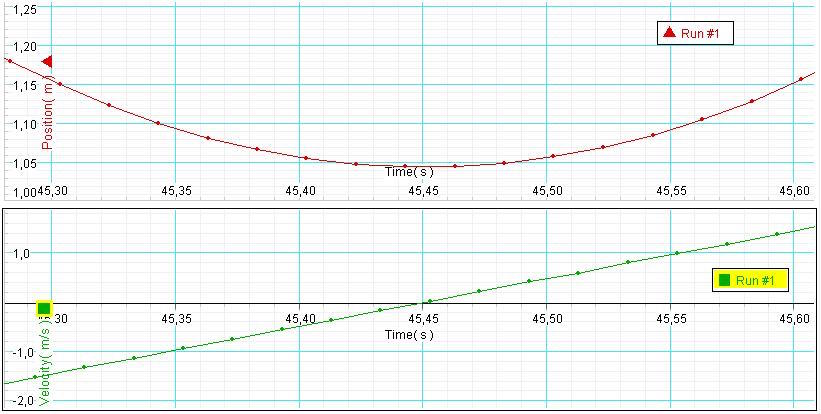
\includegraphics[width=0.9\textwidth]{valbeweging_pasco3}
\caption{Experimenteel bekomen grafieken van een verticale worp}
\end{figure}

Als we een appel laten vallen zal de zwaartekracht ervoor zorgen dat de appel naar de aarde valt. Wanneer we bovendien de snelheid meten, zien we dat deze snelheid toeneemt en wel op een constante manier. Dat wil zeggen dat er per tijdseenheid steeds evenveel snelheid bijkomt. De appel valt sneller en sneller maar de mate waarin dat gebeurt, is constant. Gooien we hem op, dan zien we dat zwaartekracht en snelheid tegengesteld zijn aan elkaar. De zwaartekracht zorgt dus duidelijk niet voor de beweging omhoog (de appel blijft omhoog gaan) maar voor een vertraging van de beweging. De snelheid waarmee de appel omhoog beweegt, neemt af. Ook hier zien we -- nadat we meten -- dat de snelheid gelijkmatig afneemt. De snelheid waarmee de appel per tijdseenheid afneemt, is steeds gelijk. Of de appel nu snel gaat of traag, de mate van afname is steeds gelijk. We kunnen dus concluderen dat de zwaartekracht voor een verandering van bewegingstoestand zorgt; de snelheid blijft niet hetzelfde. We zien zelfs dat die verandering van de snelheid gelijkmatig is. De constante zwaartekracht zorgt blijkbaar voor een constante verandering van de snelheid. 

Als je kijkt naar een koppel schoonschaatsers, dan zie je naast een fantastische prestatie en een mooi schouwspel, dat een kracht niet altijd voor een toename of afname in de grootte van de snelheid hoeft te zorgen. 
\begin{figure}[h]
\centering
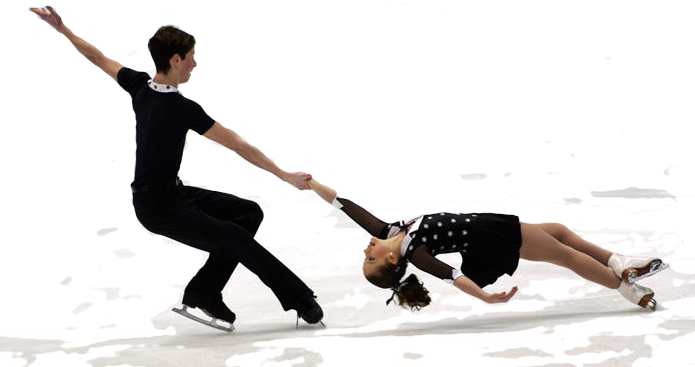
\includegraphics[width=0.7\textwidth]{schoonschaatsers2}
%\caption{A gull}
\end{figure}
De jongen in de figuur moet duidelijk een kracht uitoefenen om het meisje dat rond hem draait, bij te houden. De kracht die nu wordt uitgeoefend, dient niet zozeer voor het veranderen van de \emph{grootte} van de snelheid dan wel voor het veranderen van de \emph{richting} van de snelheid. Op elk moment verandert de richting van de snelheid, en dit naar de jongen toe -- volgens de richting van de kracht.

We kunnen concluderen dat een kracht niet zozeer invloed uitoefent op de snelheid dan wel op de \emph{verandering} van de snelheid. Deze verandering houdt zowel een verandering van grootte en/of een verandering van richting in. Bovendien blijkt uit de laatste twee voorbeelden dat de verandering te associ\"eren is met de kracht; de verandering is in de richting van de kracht. Snelheid is te beschrijven als een vector en verandering van grootte en/of richting vallen beide onder het veranderen van de vector. Als we die verandering versnelling noemen, lijkt er een relatie te zijn tussen de kracht en de versnelling -- tussen de oorzaak en het gevolg\ldots

In hoofdstuk 1 en 2 bekijken we het formalisme om bewegingen te \emph{beschrijven}. Dit onderdeel noemen we kinematica. In hoofdstuk 3 en 4 behandelen we dan het \emph{verklarende} principe achter de beweging. Dit noemen we dynamica. Het geheel -- kinematica en dynamica -- noemen we mechanica.

\clearpage
\newpage